
\section{Bayesian Neural Interconnection and Damping Assignment PBC}

In this subsection, we formulate a Bayesian learning framework that tackles the
adverse effects of system parameter uncertainties. 
%
We parametrize the function $V_d^\theta$ and the entries of $L_\theta$ and
$A_\theta$ matrices with Bayesian neural networks. 
%
We invoke variational inference to find the approximate posterior over the
parameters $\theta$. The goal is to learn the distribution parameters $z$ of the
posterior multivariate probability distribution $Q(\theta;z)$ that maximize the
\textsc{Elbo} given in~\eqref{eq:elbo}.
%


The computation of the \textsc{Elbo} requires the likelihood function and the
prior distribution.
%
In order to compute the likelihood, we first draw samples of $\theta$ from the
posterior $Q(\theta;z)$, and evaluate the PDEs given in~\eqref{eq:pde_idapbc}.
Then, the likelihood is given by
\begin{equation}
    P( \left\| l_{\textrm{IDA}} (x) \right\|^2 \mid \theta) = \mathcal{N}\left(0, s \right),
    \label{eqn:likelihood_idapbc}
\end{equation}
where $\mathcal{N}$ represents the Gaussian probability distribution, and $s$ is
a hyperparameter that represents the standard deviation of the likelihood.
%
With the choice of the likelihood function given in
\eqref{eqn:likelihood_idapbc}, maximizing the \textsc{Elbo}
in~\eqref{eq:elbo} coaxes the loss $l_{\text{IDA}}(x)$ to zero.


%
We update the distribution parameters $z$ along the gradient $\partial
\mathcal{L}/\partial z$ until the \textsc{Elbo} converges and the objective
function $\left\| l_{\textrm{IDA}} (x) \right\|^2$ reaches the threshold
$\epsilon_{tol}$.
%
We invoke the reparameterization trick of the Automatic Differentiation
Variational Inference(\textsc{ADVI})~\cite{kucukelbir2015automatic} to compute
the gradient of samples $\theta$ with respect to the distribution parameters
$z$.


System parameter uncertainties can deteriorate the performance of controllers
employed on real systems. 
%
Hence, in the Bayesian framework, we inject these uncertainties directly into
the training loop in order to learn a controller that works for a wide range of
system parameters.
%
To model these uncertainties, we sample a set of system parameters $p_s$ from
a normal distribution $\mathcal{N}(\hat{p}_s, \sigma_{p})$ centered around the
nominal parameter $\hat{p}_s$, where $\sigma_{p}$ represents the uncertainty
in system parameters.
%
Each time we compute the PDE loss $l_{\text{IDA}}$ for a batch of discrete
states sampled from the configuration space $\mathcal{Q}$, we draw a new sample
of $\zeta$.


\subsection{Inertia Wheel Pendulum}

\subsubsection{Training}
The optimization problem~\eqref{eq:idapbc_finite_optim} is constructed as
follows. The potential energy function $V_d^\theta$ is a fully-connected neural
network with two hidden layers, each of which has the activation function
\textsc{Elu}.
%
The closed-loop mass matrix is constructed according to the Cholesky
decomposition $M_d^\theta = L^\top_\theta L_\theta$, where the components of
$L_\theta$ are part of the parameters $\theta$ to be optimized.
%
We choose $J_2^\theta = 0$, as the mass matrix is independent of $q$ for
this system.
%
The parameters of the surrogates are initialized according to the Glorot
(Xavier)~\cite{glorot2010understanding} scheme.
%
The optimization problem is solved over a uniform discretization of $q = \left(
q_1, q_2 \right) \in [-2\pi, 2\pi] \times [-50, 50]$.


In the deterministic setting, the nominal system parameters reported in
Table~\ref{tab:modified_params} are used for $H(q,p)$ during training. 
%
In the Bayesian setting, the standard deviations $\sigma_{p}$ of system
parameters $p_s = [I_1, I_2, mgl]$ are chosen to be $10\%$ of the nominal system
parameters given in Section~\ref{subsec:iwp}.
%
We use variational inference to estimate a Gaussian posterior distribution
over uncorrelated parameters.
%
After training, both settings use the nominal values for the computation of
$H(q,p)$ in the control synthesis given by Equation~\eqref{eq:idapbc_ues}.
%
A summary of the hyperparameters for both the deterministic and Bayesian methods
are given in Table~\ref{tab:training_setup_idapbc}. 
\begin{table}[t]
    \centering
    \caption{\textsc{Neural-IDAPBC} training setup for deterministic and Bayesian frameworks}
    % \rowcolors{2}{}{Wheat1}
    \begin{tabular}{lcc}
    \toprule
    %   & \multicolumn{2}{c}{Framework} \\
    %   \cmidrule(lr){2-3}
    & Deterministic & Bayesian \\
    \midrule
        Neural net size & (2, 8, 4, 1) & (2, 8, 6, 1)\\
        \# of parameters &  56  & 150\\
        Optimizer & \textsc{Adam} & DecayedAdaGrad\\
        Initial learning rate & 0.001 & 0.01\\
    \bottomrule
    \end{tabular}
    \label{tab:training_setup_idapbc}
\end{table}

\subsubsection{Simulation Tests} 
The performance of the controllers obtained from the deterministic and Bayesian
trainings are compared as follows.
%
% Both frameworks are trained with the nominal system parameters given in
% Table~\ref{tab:modified_params}.
%
Similar to the \textsc{NeuralPbc} simulation tests, we introduce system
parameter uncertainties by moving the average system parameters by $\pm
10\%$ to $\pm 50\%$ with increments of $10\%$. 
%
For each average system parameter, we sample uniformly with a $\pm 5\%$ support
around the average system parameters. 
%
This helps test the performance of the controller with various combinations of
$I_1, I_2$ and $m_3$.
%
%
% On top of the system parameter uncertainties, we introduce measurement noise
% represented by a Wiener process with standard deviation of $0.005$ and $0.05$ on
% the joint angles and velocities, respectively. 
%
Figure~\ref{fig:comparison_idapbc} shows the performance of the controllers.
The policy learned from the Bayesian training is marginalized over 10
parameters sampled from the posterior per~\eqref{eqn:marginalization}.

As seen in Figure~\ref{fig:comparison_idapbc}, trajectories from the Bayesian
controller incur much lower cost than the deterministic counterpart throughout a
wide range of errors in system parameters.
%
Moreover, we observe that the error band on the cost corresponding to Bayesian
training is narrower.
%
These results show that controllers trained via Bayesian learning are
consistently more robust to errors in system parameters.
\begin{figure}
    \centering
    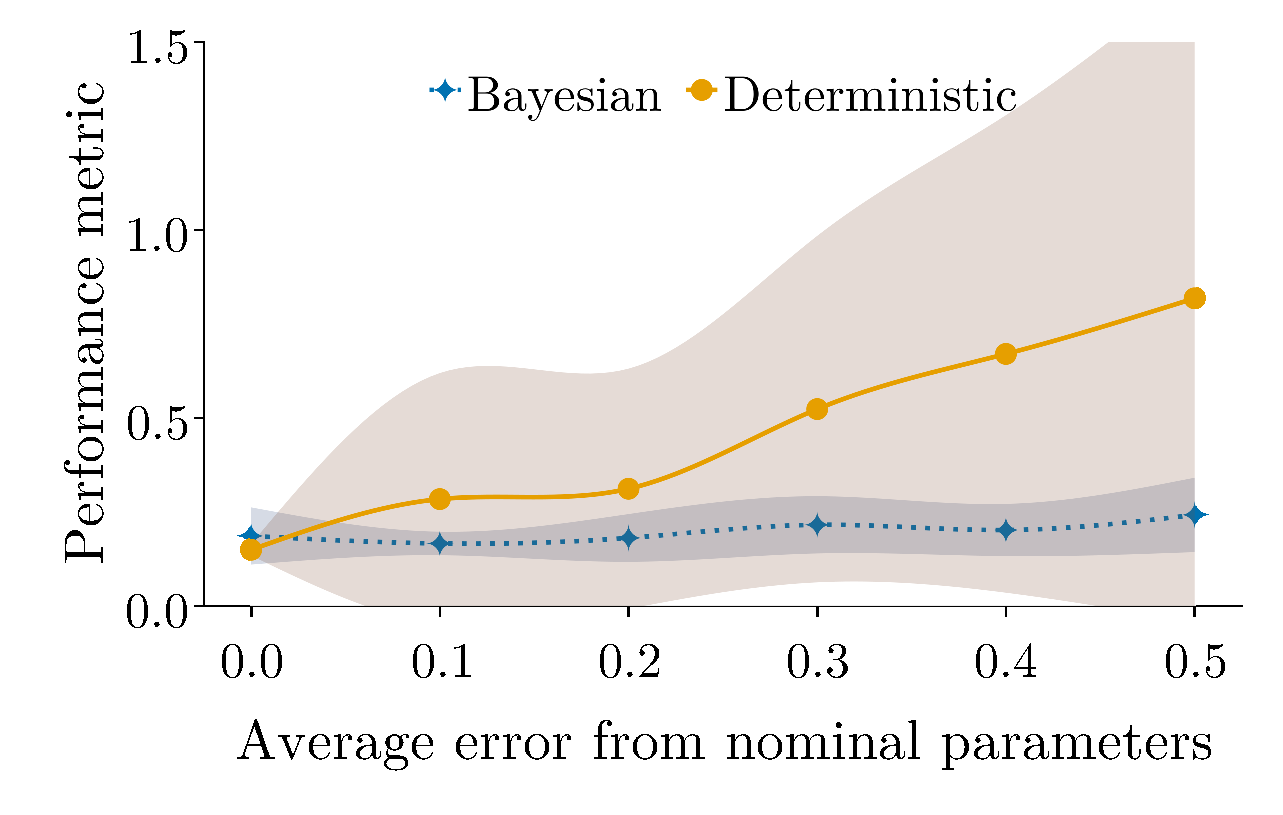
\includegraphics[clip,width=0.6\columnwidth]{./figures/bandplot1.eps}%
    \caption{
        %
        Accumulated quadratic cost ($J^T$) for a range of error in system
        parameters. 
        %
        Lower values correspond to better controller performance.
        %
    }
    \label{fig:comparison_idapbc}
\end{figure}

\subsubsection{Hardware Tests} 

The hardware experiments are designed to further demonstrate the robustness of our
controllers against model uncertainties, which include errors in the parameters,
friction in the bearings, and any contribution to the dynamics from the
belt-drive system.
%
We deliberately modify the hardware to create large errors in the model
parameters and test the controllers without any additional training.
%
In particular, the inertia wheel attached to $q_2$ is replaced with parts whose
mass and inertia values differ from the nominal values (see
Table~\ref{tab:modified_params}). The state $x$ is recorded, and the performance
metric~\eqref{eq:performance_metric} is used to evaluate the controllers.
%
The results are summarized in Figure~\ref{fig:neuralidapbc_bar_plot}.

In all scenarios, we recorded a 100\% success rate in the swing-up task despite
the errors introduced in the system parameters.
%
Furthermore, we observe that the controller from Bayesian training consistently
outperforms the deterministic counterpart, supporting the
theoretical justification discussed in Section~\ref{sec:justification}. 
\begin{figure}[H]
    \centering
    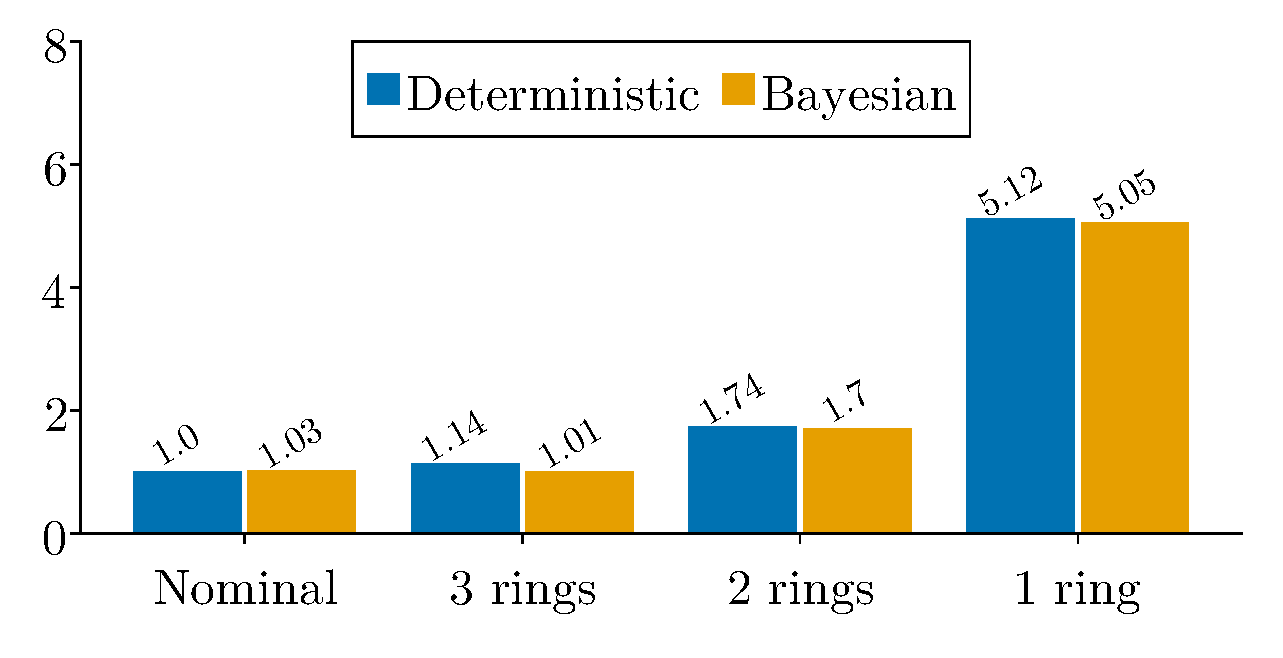
\includegraphics[width=0.6\linewidth]{./figures/idapbc_bar.eps}
    \caption{
        %
        Normalized accumulated cost $J_{T}$ (lower is better) for
        modified system parameters.
        %
        The categories A-C correspond to the parameters shown in
        Table~\ref{tab:modified_params}.
        %
    }
    \label{fig:neuralidapbc_bar_plot}
\end{figure}
%

